%Vorlage Uni, made by Oliver Wisler 25.20.2011

%set document language to german, standard font size and document size
\documentclass[ngerman, 12pt, pdftex]{scrartcl}[2006/07/30]

%encoding and input
\usepackage[ngerman]{babel} %spell correction
\usepackage[utf8]{inputenc} 
\usepackage[T1]{fontenc}
\usepackage[
	colorlinks=true,
	urlcolor=blue,
	linkcolor=green
]{hyperref}


%bugfixes
\usepackage{fixltx2e} 

%Font Symbols and Colors
\usepackage{textcomp} %more symbols
\usepackage{xcolor}

%Math
\usepackage{amsmath}
\usepackage{mathtools} %extends amsmath

%Programming
\usepackage{listingsutf8} %in utf8d
\lstset{language=Java,captionpos=b,tabsize=3,frame=lines,keywordstyle=\color{blue},commentstyle=\color{teal},stringstyle=\color{red},numbers=left,numberstyle=\tiny,numbersep=5pt,breaklines=true,showstringspaces=false,basicstyle=\footnotesize,emph={label},upquote=true} %Syntax highlighting

\usepackage{dirtree} 


%Verbatim extension (with line numbers and tab-expansion)
\usepackage{moreverb} 

%Headers and Footer
\usepackage{fancyhdr}

%title
\title{CS261 Webprojekt}
\author{Frank Müller, Oliver Wisler}

\begin{document}
%declare  Header
\pagestyle{fancy}
\fancyhf{} 
\fancyhead[L]{cs261 Webprojekt} %left header
\fancyhead[C]{Dokumentation} %centered header
\fancyhead[R]{Frank Müller, Oliver Wisler}  % right header
\renewcommand{\headrulewidth}{0.1pt} 	%upper separating line
\fancyfoot[C]{\thepage} 				%centered footer, line number
%\renewcommand{\footrulewidth}{0.1pt} 	%lower separating line




%%%%%CONTENT%%%%%
%you might want to enable come features:
%\maketitle
\tableofcontents
\newpage


\section{Installation}

Für die Installation müssen folgende Schritte durchlaufen werden:
\subsection{Installation der Dateien}
    Bitte kopieren Sie alle Dateien in das gewünschte Stammverzeichnis.
    Ihr Webserver muss PHP und MySQL unterstützen, um diese Webseite anbieten zu können. Unter Umständen müssen Sie die Pfade der Datei \verb+./.htaccess+ an Ihre Serverinstallation anpassen.
\subsection{Setzen der Konstanten}
    Setzten Sie alle wichtigen Konstanten in \verb+./config.php+.
    Die Verwendung und Bedeutung der Konstanten wird in der Datei erklärt.
    Achten Sie darauf, dass die Konstante \verb+INSTALL+ auf den Wert 1 gesetzt wird.
\subsection{Installation der Datenbank} % (fold)
\label{sub:Installation der Datenbank}
    Stellen Sie sicher, dass die in  \verb+./config.php+ angegebene Datenbank existiert.
    Führen Sie die Datei  \verb+./db_setup.php+ mit PHP aus. Alternativ können Sie auch 
    die url  \url{http://www.IhreWebsite.ch/Pfad_zu_db_setup.php/db_setup.php} aufrufen.
% subsection Installation der Datenbank (end)
\subsection{Einrichten} % (fold)
\label{sub:Einrichten}
	\paragraph{Root-Benutzer}
		Es wird ein Hauptbenutzer angelegt. Sie müssen für diesen Benutzer ein Passwort festlegen. 
		Dies geschieht mit dem Aufruf von \url{http://www.IhreWebsite.ch/Pfad_zu_setRootPass.php/setRootPass.php?passwd=IhrPasswort}.
		Ersetzen Sie \verb+IhrPasswort+ mit einem sicheren Passwort.
	\paragraph{Installation abschliessen}
		Nun können Sie die Konstante \verb+INSTALL+ auf 0 setzen. Die Installation ist somit abgeschlossen.
    
  


% subsection Einrichten (end)


% section  (end)

\section{Umsetzung}
\subsection{Funktionsumfang}


% subsection  (end)
\subsection{Aufbau}
	\subsubsection{Dateisystem}
\dirtree{%
 .1 /. 
 .2 installfiles\DTcomment{Installationsdateien}. 
 .2 templates\DTcomment{Vorlagen für die Seiten}. 
 .2 css\DTcomment{CSS Dateien}. 
 .2 js\DTcomment{Javascript Dateien}. 
 .2 handlers\DTcomment{Ajax Handler}. 
 .2 img\DTcomment{Bilder}. 
 .2 uploads\DTcomment{Hochgeladene Dateien}. 
 .2 doc\DTcomment{Dokumentation}. 
}
		
	\subsubsection{Seitenaufbau}
	\lstset{language=html}
\begin{lstlisting}
<html>
	<head>
		<!-- Hier sind alle CSS Dateien eingebunden -->
	</head>
	<body>
		<div id="content">
			<header>
				<!-- Hier ist das Menu -->
			</header>
			<!-- Benachrichtigungsfeld -->
			
			<article>
				<!-- hier ist der verlangte Seiteninhalt -->
			</article>
					
					
		</div>
		<!-- Hier sind alle Javascritp Dateien eingebunden -->
	</body>
</html>
	\end{lstlisting}
	
	\subsubsection{Benutzerführung}
 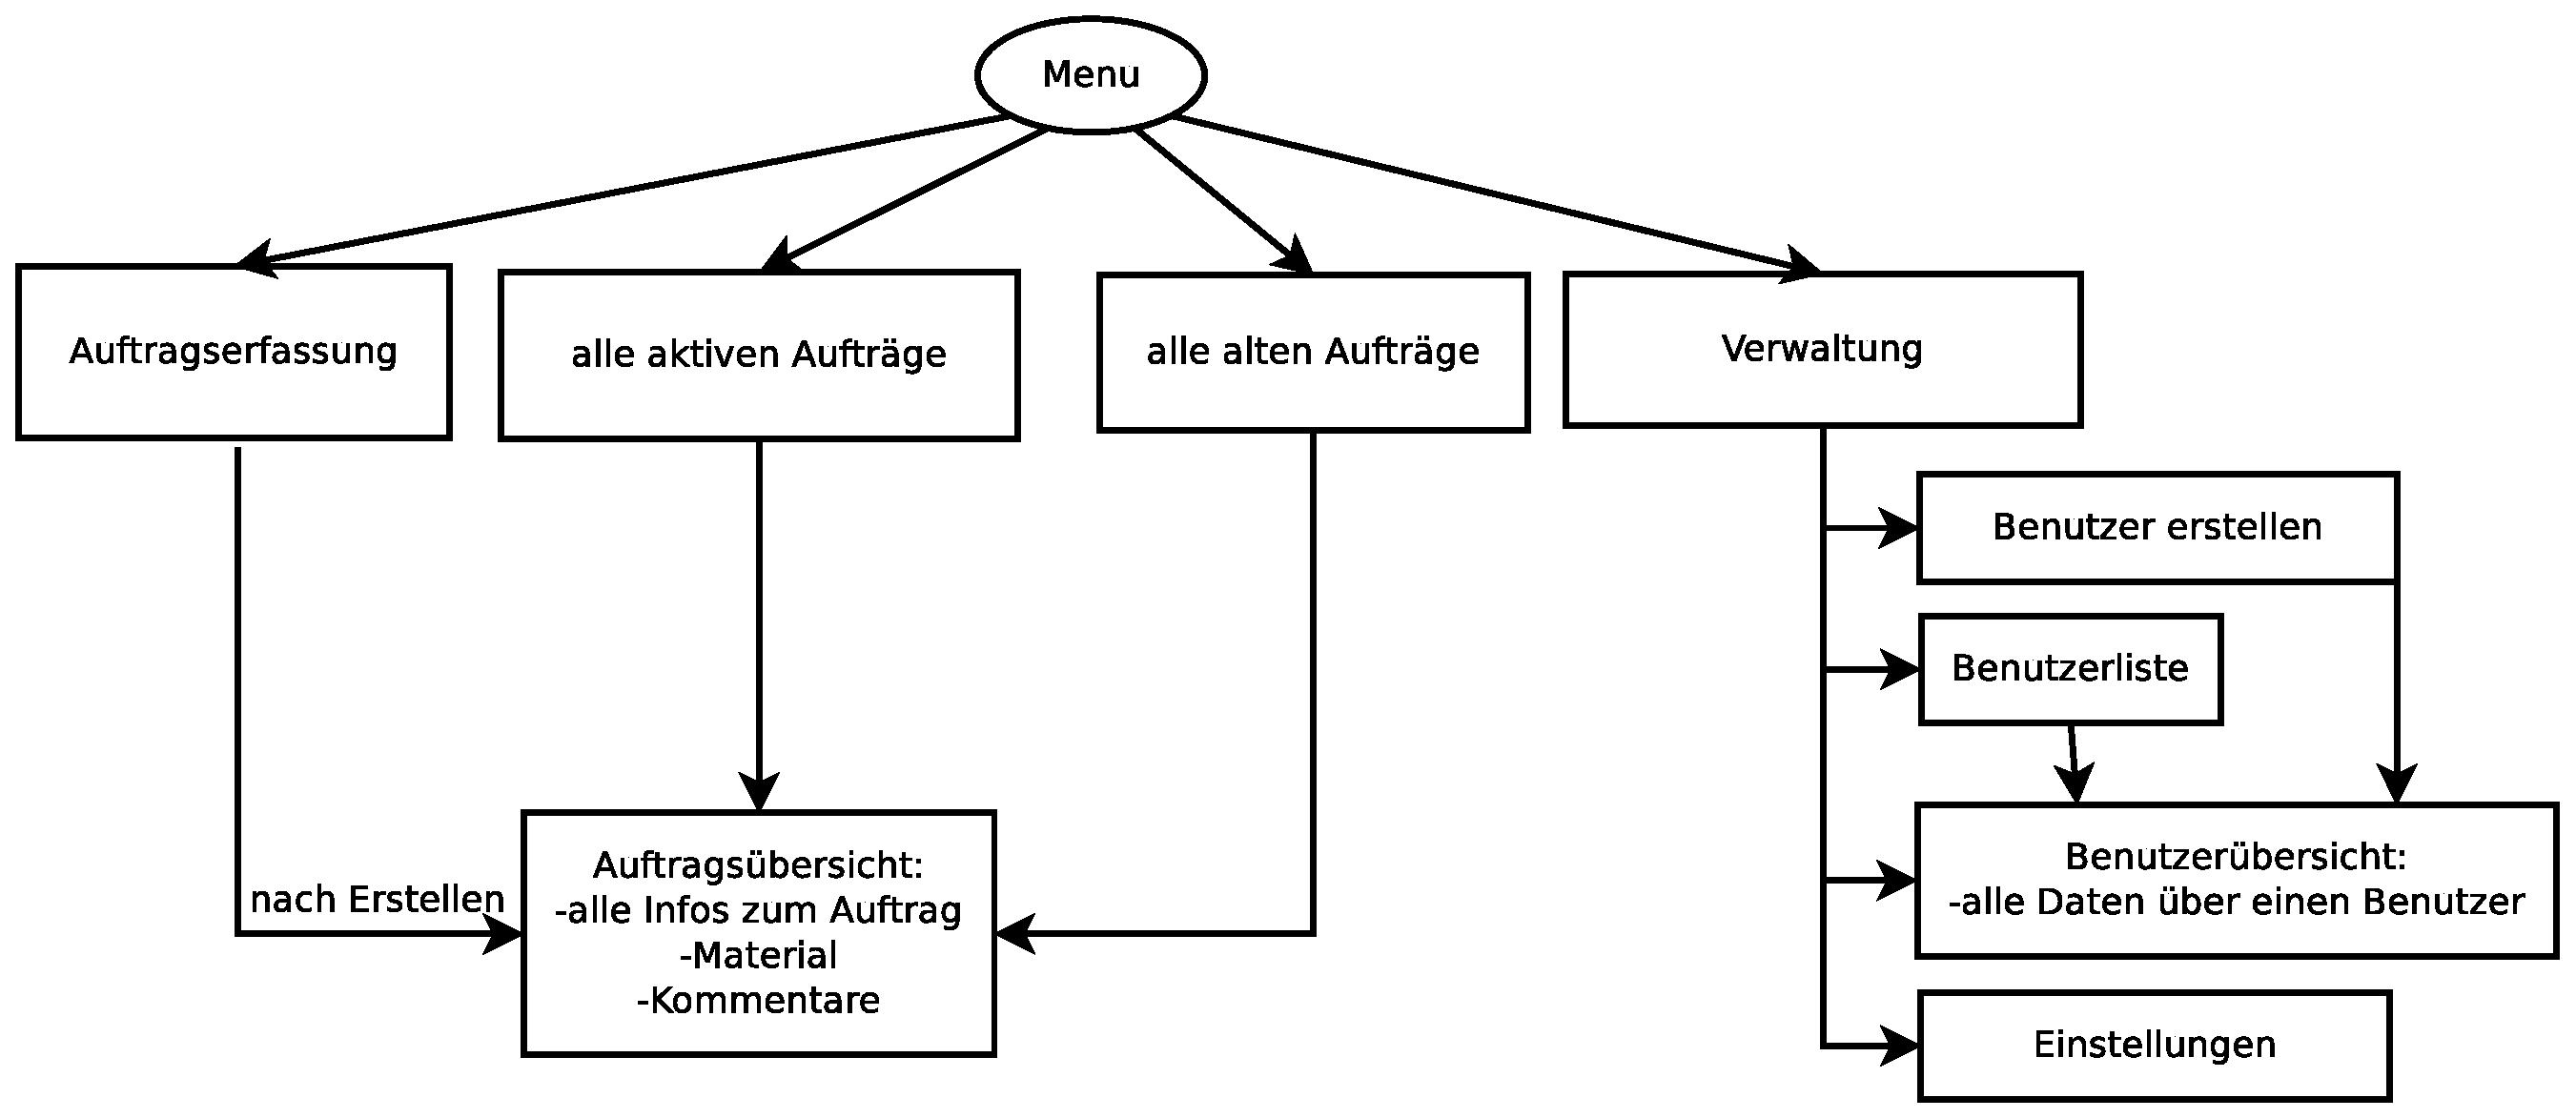
\includegraphics[width=\textwidth]{navigation.eps}

% subsection  (end)
\subsection{Datenbank}


% subsection  (end)
% section  (end)
\subsection{Verwendete Komponenten und Bibliotheken} % (fold)
\begin{itemize}
\item jQuery \url{http://jquery.com/}
\item Iconic \url{https://github.com/somerandomdude/Iconic}
\item SuperBox \url{http://pierrebertet.net/projects/jquery_superbox/}
\item tinyMCE \url{www.tinymce.com/}
\item AjaxFileUploader \url{https://github.com/jfeldstein/jQuery.AjaxFileUpload.js}
\end{itemize}



\section{Benutzeroberfläche}
\subsection{Verwaltung}

% subsection  (end)
\subsection{Lagerist}


% subsection  (end)

\subsection{Arbeiter}


% subsection  (end)
% section  (end)

\section{Fazit}
\subsection{Einschränkungen}

% subsection  (end)
\subsection{Problemstellen}

% subsection  (end)
\subsection{Lessons learned}

% subsection  (end)

% section  (end)
\end{document}]
